\chapter{Controller description} 
\label{cha:description}

This chapter contains a description of the controller strategy, architecture, filters, parameters, and in-/outputs. The controller is a further development of a previous controller used at DTU Wind Energy under the version 11. The new developments are inspired by Bossanyi's controller for the 5MW NREL reference turbine \cite{Bossanyi09}, where the power error feedback in the pitch controller that keeps the pitch at its minimum below rated power operation represents the most significant change.

Compared to the previous release of the Basic DTU Wind Energy controller, the main improvements of the current version include a rotor speed exclusion zone, a tower damper, a new formulation of the drivetrain damper, and a controller for operation in storm wind conditions. 

The controller is only considering low speed shaft (LSS) measures of rotational speeds and torques, i.e., there is no gearbox on the drivetrain. The controller can still be used for turbines with a gearbox, when the user transforms torques and speeds between the LSS and HSS using the gear ratio.

\section{Strategy and architecture}

A diagram of the entire controller is shown in Figure~\ref{f:diagram}. The routes of this diagram that are active when the turbine is operating below rated power, herein called \emph{partial load} operation, are shown in Figure~\ref{f:diagram_part}. The routes that are active in \emph{full load} operation are shown in Figure~\ref{f:diagram_full}. These two regions of operation are first described before the switching between is explained. The discrete filters denoted by the functions $f_1$, $f_2$, and $f_n$ in the diagrams are described and tested in Appendix~\ref{ch:filters}. The appendix also illustrates a band-pass filter denoted $f_p$.

\subsection{Partial load operation}

The strategy for optimal $C_P$ tracking in partial load operation is based on a balance between generator and aerodynamic torques to obtain a close to optimal tip speed ratio. To avoid the feedback of higher frequency dynamics (e.g. the drivetrain torsion mode), the torque reference $Q_{ref,k}$ at the current step $k$ is computed based on a second order low-pass filtered LSS generator speed as $K \bar \Omega_k^2 - K_{dot} \dot{\bar \Omega}_k$. This feedback is enforced by setting the torque limits for the PID controller to $Q_{g,min,k}=Q_{g,max,k}=K\bar \Omega_k^2 - K_{dot} \dot{\bar \Omega}_k$ whenever the filtered rotational speed $\bar \Omega_k$ is not close to the minimum speed $\Omega_{min}$, or the rated speed $\Omega_0$. When the rotational speed is close to its bounds, these torque limits will open according to the interpolation factors $\sigma_{min,k}$ and $\sigma_{max,k}$. The torque reference will then be given by the PID controller based on the speed error $e_{Q,k}=\bar\Omega_k -\Omega_{set,k}$, where the set point is the minimum, or rated speed. Because the rotor speed is bounded, the power loss can often be minimized be performing some adjustment of the minimum pitch. A first order low-pass filtered wind speed measured at hub height $\bar V_k$ is used as parameter for varying the minimum pitch angle $\theta_{min,k}=\theta_{min}(\bar V_k)$ based on a look-up table provided by the user. The power error feedback of pitch PID controller ensures that the pitch reference is kept at this minimum pitch angle.

\begin{sidewaysfigure}
\centerline{\epsfig{figure=discrete_diagram.eps,width=1.05\textheight} }
\caption{Diagram of the discrete controller. Note that $k$ denotes the current time step. \label{f:diagram}}
\end{sidewaysfigure}

\begin{sidewaysfigure}
\centerline{\epsfig{figure=discrete_diagram_part.eps,width=1.05\textheight} }
\caption{Active routes during partial load operation in the controller diagram in Figure~\ref{f:diagram}. \label{f:diagram_part}}
\end{sidewaysfigure}

\begin{sidewaysfigure}
\centerline{\epsfig{figure=discrete_diagram_full.eps,width=1.05\textheight} }
\caption{Active routes during full load operation in the controller diagram in Figure~\ref{f:diagram}. \label{f:diagram_full}}
\end{sidewaysfigure}

The interpolation factors for the opening of the torque limits are based on how close the second order low-pass filtered generator speed is from its minimum and rated speeds. The limits can be opened gradually over an interval as described by the function
\begin{equation}\label{e:sigma}
\sigma\left(x_0,x_1;x\right) = \left\{
\begin{array}{rl}
0 & \forall x<x_0 \\
a_3x^3 + a_2x^2 + a_1x + a_0& \forall x\in[x_0:x_1[\\
1 & \mbox{otherwise}
\end{array} \right.
\end{equation}
where the coefficients of the spline are
\begin{equation}\label{e:sigmacoef}
a_3=\frac{2}{\left(x_0-x_1\right)^3}, \;\;\;\;
a_2=\frac{-3 \left(x_0+x_1\right)}{\left(x_0-x_1\right)^3}, \;\;\;\;
a_1=\frac{6 x_1 x_0}{\left(x_0-x_1\right)^3}, \;\;\;\;
a_0=\frac{\left(x_0-3 x_1\right) x_0^2}{\left(x_0-x_1\right)^3}
\end{equation}
The function is programmed such that if $x_0 \geq x_1$ then the $\sigma$-function becomes
\begin{equation}\label{e:sigma_if}
\sigma\left(x_0,x_0;x\right) = \left\{
\begin{array}{rl}
0 & \forall x<x_0 \\
1 & \mbox{otherwise}
\end{array} \right.
\end{equation}
Figure~\ref{f:sigma} shows an example of the $\sigma$-function where $x_0=1$ and $x_1=2$. In an actual implementation of the controller, this smooth function with a third order polynomial may be an unnecessary complexity, which can been replaced by a linear interpolation function.

Figure~\ref{f:torque_limits} shows the torque limits in partial load operation of the DTU 10~MW RWT, where the minimum speed is 5~rpm and rated speed is 9.6~rpm. Several operational regions can be seen here. Namely the bellow minimal rotational speed region, variable speed region with exclusion zone functionality, transient variable to constant speed region and finally constant speed region. The generator torque limits are set to be open in bellow minimal rotor speed, where the maximal torque limit is set to
\begin{equation}\label{e:Tg_blw_min_w}
Q_{g,max} = \max\left\{
\begin{array}{l}
K \Omega_{min}^2 \\
K \bar\Omega_k^2 - K_{dot} \dot{\bar \Omega}_k
\end{array} \right.
\end{equation}
%$Q_{g,max}= K\dot\Omega_{min}^2$
and minimal torque is equal to zero. The generator torque limits are closed approximately 5~\% above the minimum speed $\Omega_{min}$ and start opening again at 90~\% and are fully open at 95~\% of the rated speed. If the exclusion zone functionality is active, the torque limits starts to open at 99~\% of the exclusion zone minimal speed $\omega_{L}$ and are closed  1~\% above the exclusion zone maximal speed $\omega_{H}$. Where the spline function is used to guarantee smooth transient. The maximal torque limit is set to $Q_{g,max}$ 5~\% above the $Q_{g_{\Omega_{L}}}$ and the minimal torque is set to $Q_{g,min}$ 95~\% of the $Q_{g_{\Omega_{H}}}$.

\begin{figure}[t]
\centerline{\epsfig{figure=sigma.eps,width=0.45\textheight} }
\caption{Example of the $\sigma$-function \eqref{e:sigma} where $x_0=1$ and $x_1=2$. \label{f:sigma}}
\end{figure}

\begin{figure}[t]
\centerline{
\epsfig{figure=torque_limits_rsa.eps,width=0.6\textwidth} }
\caption{Torque limits in partial load operation of the DTU 10~MW RWT, where the minimum speed is 5~rpm and rated speed is 9.6~rpm. The limits are set to be closed approximately 5~\% above the minimum speed and start opening again at 90~\% and are fully open at 95~\% of the rated speed. \label{f:torque_limits}}
\end{figure}

\subsection{Full load operation}

In full load operation, the torque limits are closed around the torque given by the selected power control strategy, either constant power $P_0/\Omega_k$, or constant torque $P_0/\Omega_0$, where $P_0$ is the rated power. Note that the unfiltered measured LSS generator speed $\Omega_k$ is used for computation of the reference torque in the constant power control.

The pitch reference angle is obtained from a combined PI feedback of the generator speed and power errors, and a possible differential feedback of the speed error. The speed error is obtained as the difference between the second order low-pass filtered LSS generator speed and the rated speed. The power error is the difference between the reference power $P_{ref,k}=Q_{ref,k}\Omega_k$ and the rated power $P_0$. Both errors are notch filtered around the frequency specified by the user as the free-free drivetrain frequency. This frequency is assumed to be constant although HAWCStab2 eigenvalue analysis often show a small variation with operational point (wind speed). Note that both errors contribute to the same proportional term ($\theta_{P,k}$) and same integral term ($\theta_{I,k}$). The latter is important because it ensures that the reference pitch angle is kept at the minimum pitch angle until rated power is reached; assuming that the right weighting between the integral speed error gain $k_{I,0}$ and power error gain $k_I^P$ has been selected by the user.

The anti-windup is performed such that the controller will react quickly with increased pitch angle if the reference power signal suddenly increased above the rated power level. In each time step, the minimum pitch limit is enforced on the reference pitch which is the sum of the proportional, differential, and integral terms $\theta_{ref,k}=\max\left(\theta_{min,k},\theta_{P,k}+\theta_{D,k}+\theta_{I,k}\right)$. The value of the integral term to be used for the integration in the next time step is then recalculated as $\theta_{I,k}=\theta_{ref,k}-\theta_{P,k}-\theta_{D,k}$, which only makes a change to the integral term if the reference pitch is on the minimum limit $\theta_{ref,k}=\theta_{min,k}$. Below rated power, where the proportional term is negative because the rotational speed error is kept close to zero by the torque PID controller, the integral term will therefore be positive. If the reference power is increased and becomes close to rated power (due to the reaction of the torque PID controller to an increased wind speed), then the proportional term will then come close to zero whereas the integral will still be positive and the resulting pitch reference angle will be positive, whereby large power and speed variations are avoided. Note that the same anti-windup scheme is used in the torque PID controller.

The first order low-pass filtered mean of the blade pitch angles $\bar \theta_{m,k}$ is used for scheduling of the gains of the pitch PID controller. A quadratic dependency of the aerodynamic torque gain with collective pitch angle is assumed as
\begin{equation}\label{e:gainsch}
\frac{\partial Q_A}{\partial \theta}= \left. \frac{\partial Q_A}{\partial \theta}\right|_{\theta=0}\left(1 + \frac{\theta}{K_{1}} + \frac{\theta^2}{K_{2}}\right)
\end{equation}
where $Q_A$ denotes the aerodynamic torque, $\theta$ is the collective pitch angle, and $\left. \frac{\partial Q_A}{\partial \theta}\right|_{\theta=0}$ is the aerodynamic gain at zero pitch. The parameters of this expression $K_1$ and $K_2$ can be obtained from curve fitting to the derivative of the aerodynamic torque with respect to collective pitch angle assuming quasi-steady aerodynamics and \emph{frozen wake} (constant induced velocities) as
\begin{equation}\label{e:dqadt}
\frac{\partial Q_A}{\partial \theta} = \frac12 \rho B \int_0^R c(r) U(r)^2 \left(
  C_L'(\alpha(r)) \sin \varphi(r)
- C_D'(\alpha(r)) \cos \varphi(r) \right) r dr
\end{equation}
where $B$ is the number of blades, $R$ is the outer radius of the rotor, $c(r)$ is the radial chord distribution, $U(r)$ is the mean steady state relative inflow velocity along the blade, $C_L'$ and $C_D'$ are the gradients of the lift and drag coefficient curves evaluated at the mean steady state angle of attack $\alpha(r)$ along the blade, and $\varphi(r)$ is the spanwise distribution of inflow angles relative to the rotor plane.

An additional term of the gain-scheduling can be activated to take into account the variation of the aerodynamic damping. A quadratic dependency is assumed also in this case

\begin{equation}\label{e:gainsch_omega}
\frac{\partial Q_A}{\partial \Omega}= \left. \frac{\partial Q_A}{\partial \Omega}\right|_{\theta=0}\left(1 + \frac{\theta}{K_{\Omega\,1}} + \frac{\theta^2}{K_{\Omega\,2}}\right)
\end{equation}
A detailed description of this scheme is described by Tibaldi~et~al.~\cite{tibaldi_effects_2014}.

Figure~\ref{f:gainsch} shows the aerodynamic torque gradients obtained from HAWCStab2 for the DTU 10~MW RWT together with the fit of the quadratic expressions \eqref{e:gainsch} and \eqref{e:gainsch_omega}. The fitted parameters are shown as inputs number 21, 22, 51, and 52 in Table~\ref{t:init} of Section~\ref{s:par}. Often, a linear fit is sufficient and it is assumed when the user enters $K_2=0$ (note that $K_1$ then is the angle where the aerodynamic gain is doubled). The gain scheduling factor based on the filtered mean pitch angle $\eta_{A,k}$ is the inverse of the expression in the parenthesis of \eqref{e:gainsch}. A nonlinear gain factor $\eta_{nl,k}$ based on the generator speed error is also added for increased sensitivity of the pitch PID controller by large speed excursions.


\begin{figure}[!t]
\begin{center}
\parbox{0.45\columnwidth}{\mbox{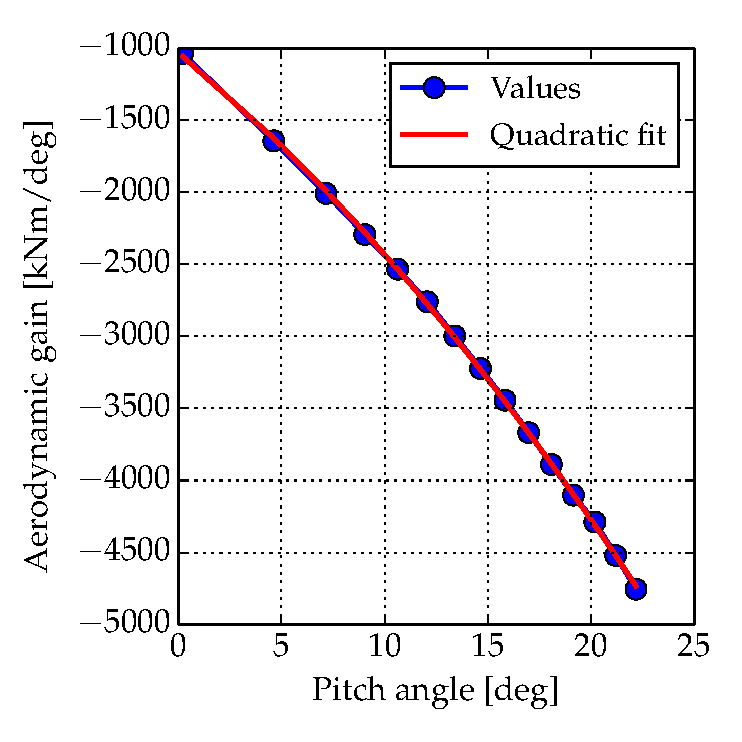
\includegraphics[keepaspectratio=true,width=0.45\columnwidth]{AG}}\center{\textit{a) Aerodynamic gainl}}}\quad
\parbox{0.5\columnwidth}{\mbox{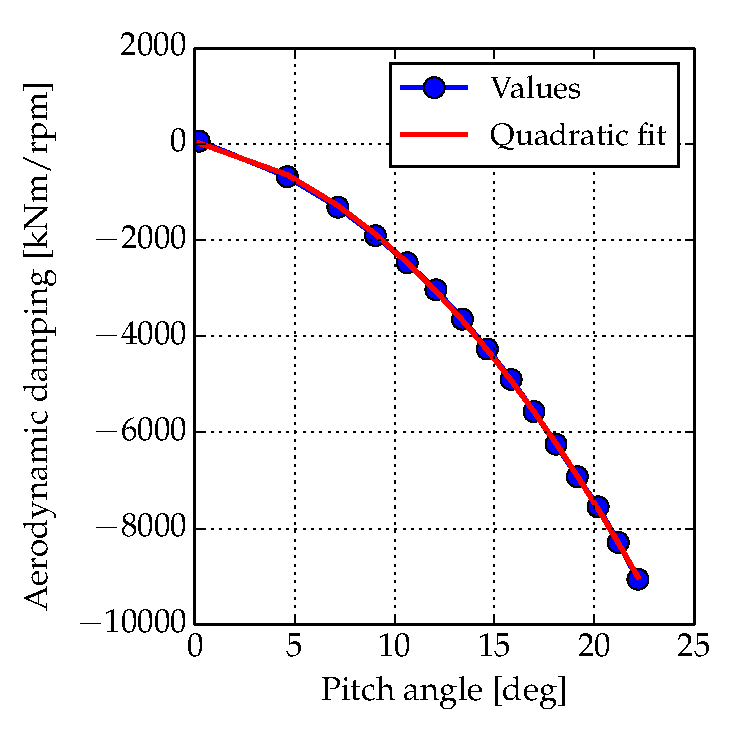
\includegraphics[keepaspectratio=true,width=0.45\columnwidth]{AD}}\center{\textit{b) Aerodynamic damping}}}
\caption{Aerodynamic gain and aerodynamic damping for the DTU 10~MW RWT. Queasi-steady values computed with HAWCStab2 and quadratic fitting.}\label{f:gainsch}
\end{center}
\end{figure}

\subsection{Switching between partial and full load operation}

The switching between partial and full load control of the generator torque is based on a first order low-pass filtered switching variable $\sigma_{\theta,k}$ that is driven by a $\sigma$-function evaluation using the measured mean pitch angle $\theta_m$. The time constant is the rotational period at rated speed. As explained above, the anti-windup of the combined integral term of the pitch PID controller will ensure that the reference pitch angle raises above its minimum value when the torque PID controller of generator speed results in a reference power close to the rated power level. The user can define at how many degrees above the minimum pitch this switching shall occur. Good experiences have been obtained with a hard switch at $\theta_{f_1}=\theta_{f_2}=\theta_{min,k}+0.5$~deg.

\subsection{Dampers}
Two dampers are part of the controller, one to reduce drivetrain vibrations and one to reduce longitudinal tower vibrations.
The dampers have the same structure. They are formed as a series of a bandpass filter, a notch filter, and a time delay. 
The bandpass filter isolates the desired frequency to damp. The notch filter further reduces the component of the signal at the frequency of a mode that could be excited by the damper. The time delay compensates the phase shift due to the signal processing and system phase lag.
The filtered signal is then multiplied by a factor to scale the damping effects.

\subsubsection{Drivetrain damper}
\label{s:dmp}

The drivetrain damper receives as input the unfiltered measured generator LSS speed $\Omega_k$.

The band-pass filter has the center frequency equals to the free-free drivetrain torsional frequency $\omega_{dt}$.
The notch filter has center frequency of $\omega_{n,dtd}$. 

The filtered speed $\Omega_{d,k}$ is multiplied by a gain factor $k_{dmp}$ and added to the torque feedback from the PID controller to give the generator torque reference. Note that this drivetrain damper is always active when $k_{dmp}\ne0$. 


The performance of drivetrain damper can bee seen from Figure~\ref{f:DT_damper}, where the vibration of the drivetrain mode are actively reduced by the damper.

\subsubsection{Longitudinal tower damper}
\label{s:TTdmp}


The measured tower top longitudinal acceleration $a_{TT}$ is used as input to the longitudinal tower damper.

The band-pass filter has the center frequency equals to the longitudinal tower mode frequency $\omega_{bp,td}$ and damping $\zeta_{bp,td}$.
The notch filter has center frequency of  $\omega_{n,td}$ and damping $\zeta_{n,td}$. 

The gain of the tower damper is defined as $k_{td}$.

The performance of the longitudinal tower damper can bee seen from Figure~\ref{f:TT_damper}, where the vibration of the first longitudinal tower mode are actively reduced.

\subsection{Exclusion zone}
\label{s:EZ}

The exclusion zone functionality avoids resonant conditions between the 3P excitation and the first lateral tower mode. The functionality logic is based on a finite-state machine with diagram presented in Figure~\ref{f:EZ_SD}. States $0$ and $3$ are variable rotor speed regimes below the exclusion zone minimal speed and above the exclusion zone maximal speed respectively. States $1$ and $2$ are constant rotor speed regimes, where the speed is stabilized on $\Omega_L$ or $\Omega_H$ by appropriate switching of the reference speed of the generator torque PID controller. During transients from state $1$ to state $2$ and other way around, the reference speed switch is low-pass filtered with a first-order filter with time constant $\tau_{EZ}$. The torque dependency on rotor speed can be seen from Figure~\ref{f:EZ_torque}. Finally the exclusion zone functionality can be seen from Figure~\ref{f:EZ}, where the rotor speed, tower top fore-aft and side to side acceleration is displayed for active and deactivated exclusion zone.

\begin{figure}[t]
\centerline{
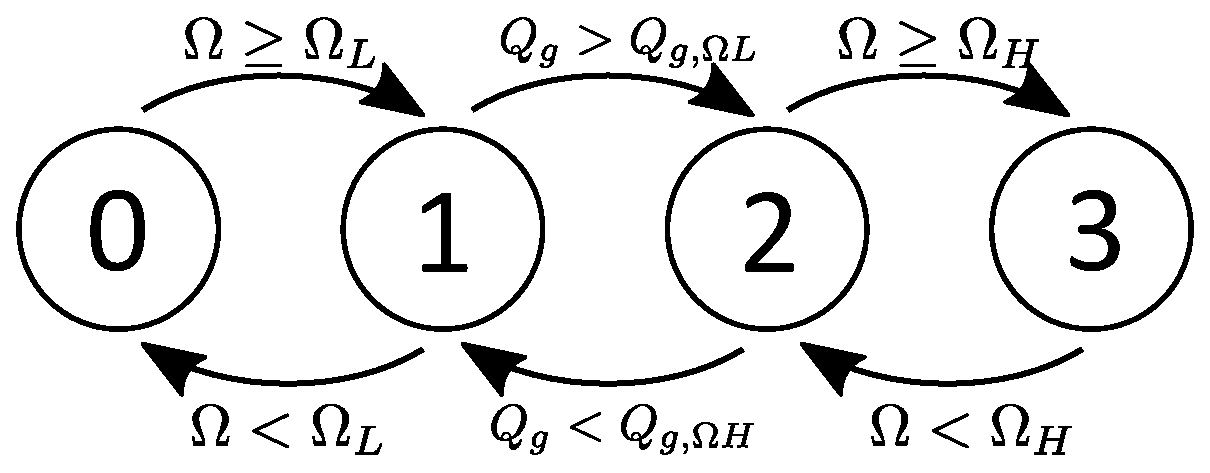
\includegraphics[width=0.4\textwidth]{ExclZone_state_diagram.eps} }
\caption{Exclusion zone logic diagram. \label{f:EZ_SD}}
\end{figure}

\begin{figure}[t]
\centerline{
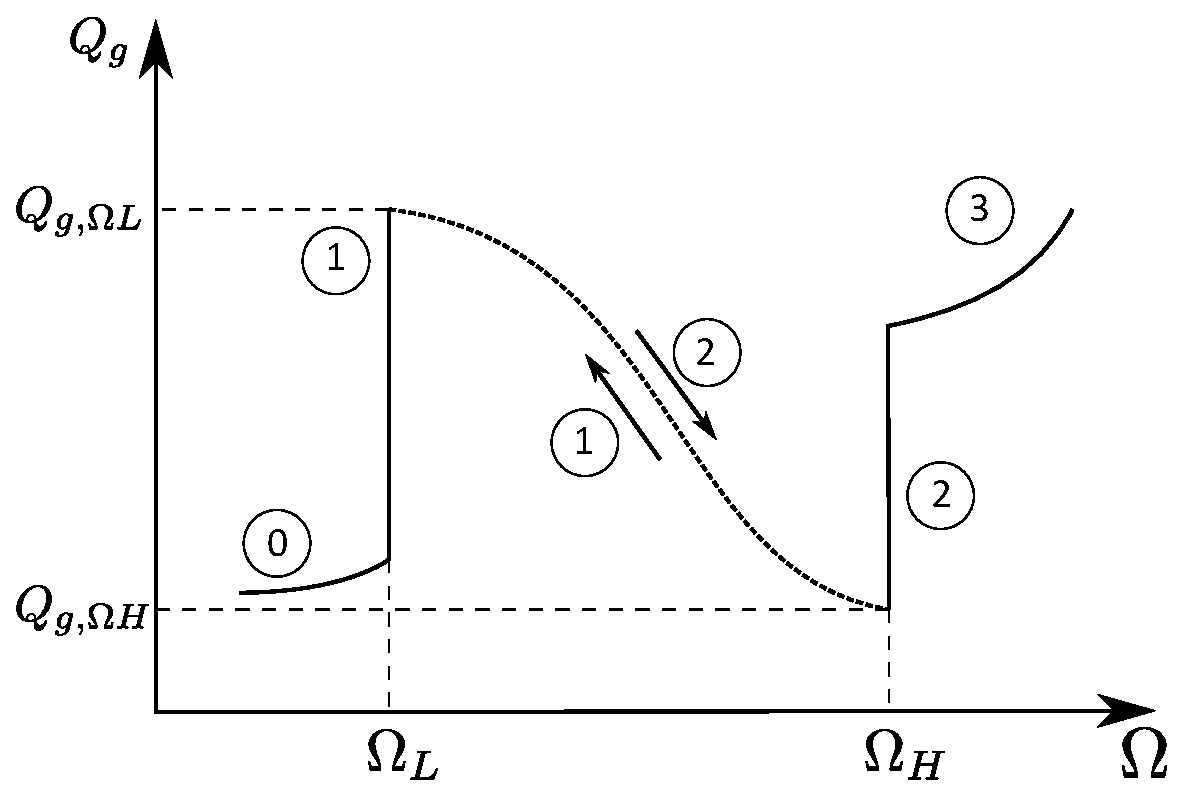
\includegraphics[width=0.6\textwidth]{ExclZone_torque.eps} }
\caption{Exclusion zone torque curve. \label{f:EZ_torque}}
\end{figure}





%\subsection{Thrust peek shaving}
%\label{s:TPS}

%The aerodynamic thrust force has its maximum closed to rotor rated speed $\Omega_0$, where the wind speed reaches its maximum for collective pitch angle at its minimal value (see \ref{f:Ft_ws}, blue curve). This introduces high extreme and fatigue loading for several wind turbine sub-components. The thrust force response to the blade pitching has negative trend (for particular wind speed, with increasing pitch angle the thrust force is reduced) and therefore collective pitch angle can be used to reduce maximal thrust. However the power production of wind turbine is also reduced as collective pitch angle differ from optimal one. Hence it is important to keep the thrust reduction to power reduction trade off in mind during thrust peek shaving design. The thrust peek shaving functionality can be implemented as altered minimal pitch angle lookup table, where higher pitch angle would be required as wind turbine approaches rated wind speed. The thrust peek shaver is implemented by dis-engaging of power error feedback loop for pitch PID, in case of DTU10MW offshore controller. This results in natural increase of pitch activity right before wind turbine hit rated wind speed. The comparison of collective pitch angle as function of wind speed, with and without thrust peek shaving function, can be seen from Figure~\ref{f:pitch_ws}.

%\begin{figure}[t]
%\centerline{
%\includegraphics[width=0.9\textwidth]{Ft_ws.pdf} }
%\caption{Thrust force as function of wind speed. \label{f:Ft_ws}}
%\end{figure}

%\begin{figure}[t]
%\centerline{
%\includegraphics[width=0.9\textwidth]{pitch_ws.pdf} }
%\caption{Collective pitch angle as function of wind speed. \label{f:pitch_ws}}
%\end{figure}


\subsection{Additional non-linear pitch control term}

This term should only be active during extreme event where severe over-speed can occur.

\begin{align}
	\dot{\theta}_{+} &= \dot{\theta}_{+} + k_{os} ( \dot{\bar{\Omega}}_k/\Omega_{os} + e_{\Omega,k}/\dot{\Omega}_{os} ) &\text{ for } ( \dot{\bar{\Omega}}_k/\Omega_{os} + e_{\Omega,k}/\dot{\Omega}_{os} ) > 1 \\
	\dot{\theta}_{+} &= \dot{\theta}_{+} &\text{ for } ( \dot{\bar{\Omega}}_k/\Omega_{os} + e_{\Omega,k}/\dot{\Omega}_{os} ) \leq 1	
\end{align}

This control block is only active if ($\Omega_{os}$,$\dot{\Omega}_{os}$,$k_{os}$) $\neq$ 0.

\subsection{TSR tracking}
Partial load regulation can be performed also tracking a constant TSR with a PID controller on the generator torque based on rotor speed feedback. The rotor speed error is calculated as $e_{Q,k}=\bar\Omega_k -\bar V_k \frac{\lambda_{opt}}{R}$, where $\bar V_k$ is the low-pass filtered wind speed, $\lambda_{opt}$ is the reference tip speed ratio, and $R$ is the rotor radius. In this case, the torque limits are kept open to allow torque values up to  $P_0/\Omega_0$.

\subsection{Storm control}
The controller includes also a feature for regulation above the standard cut-out wind speed, i.e. in storm conditions. The reference rotational speed $\Omega_{set, k}$ used for the pitch regulation is linearly reduced, based on a low-pass filtered measurement of the wind speed. The reduction goes from the rated rotational speed value ($\Omega_0$) at the standard cut-out wind speed, now defined as storm wind speed ($V_{storm}$), to the minimum allowed rotor speed value ($\Omega_{min}$) at a new cut-out wind speed ($V_{cut-out}$). The generator torque is kept at its rated value.


\section{Parameters}
\label{s:par}

All parameters of the controller are transferred to the DLL using HAWC2 commands for the \verb|init_regulation| routine of the type2 DLL \cite{Larsen12}. Details of all 52 parameters are given in Table~\ref{t:par}, where the notation of the parameters used in the diagram of Figure~\ref{f:diagram} and some additional notations can also be seen. Additional features can be enabled by using the \verb|init_regulation_advanced| instead, this routine requires 75 parameters, where the first 52 are identical to those of \verb|init_regulation|. The additional parameters can be found in Table~\ref{t:par2}.

\begin{table}[!htbp]
\begin{center}
\begin{tabular}{r|c|p{11.5cm}}
Input &  & Additional explanation if assumed needed \\ \hline
1 & $P_0$ 			& Rated power [kW].\\
2 & $\Omega_{min}$	& Minimum rotor speed [rad/s].\\
3 & $\Omega_0$ 		& Rated rotor speed [rad/s]. \\
4 & - 				& Maximum allowable generator torque [Nm]. An upper limit set on the torque reference signal. \\
5 & - 				& This number is the minimum pitch angle $\theta_{min}$ in degrees, which is set to a constant if this input is less than 90~deg. Otherwise, the init routine will search for a file with the name ``wptable.n'', where ``n'' is a character string obtained from the integer value of the input. In the shown example, this file is therefore ``wptable.100''. The file format is first line contains an integer with the number of subsequent lines, which contain two numbers each, wind speed and minimum pitch angle in degrees. An example is shown in Table~\ref{t:wptable}.\\
6 & $\theta_{max}$	& Maximum pitch angle [deg]. \\
7 & - 				& Maximum pitch velocity operation [deg/s]. An upper limit set on the rate of change of the pitch reference signal.\\
\hline
8 & $\omega_{\Omega}$ 	& Frequency of generator speed filter [Hz]. \\
9 & $\zeta_{\Omega}$ 	& Damping ratio of speed filter [-]. \\
10 & $\omega_dt$ 		& Frequency of free-free DT torsion mode [Hz], used for a notch filter and a band-pass filter of the damper. \\
\hline
11 & $K$ 			& Optimal $C_P$ tracking factor [Nm/(rad/s)$^2$], $K=\eta \frac12 \rho A C_{P,opt} R^3/\lambda_{opt}^3$. \\
12 & $k_P^g$ 		& Proportional gain of torque controller [Nm/(rad/s)]. \\
13 & $k_I^g$ 		& Integral gain of torque controller [Nm/rad]. \\
14 & $k_D^g$ 		& Differential gain of torque controller [Nm/(rad/s$^2$)]. \\
15 & - 			& Generator control strategy [1=constant power, 2=constant torque]. \\
16 & $k_{P,0}$ 		& Proportional gain of pitch controller [rad/(rad/s)]. \\
17 & $k_{I,0}$ 		& Integral gain of pitch controller [rad/rad].\\
18 & $k_{D,0}$ 		& Differential gain of pitch controller [rad/(rad/s$^2$)]. \\
19 & $k_P^P$ 		& Proportional power error gain [rad/W]. \\
20 & $k_I^P$ 		& Integral power error gain [rad/(Ws)]. \\
21 & $K_1$ 			& Coefficient of linear term in aerodynamic gain scheduling [deg]. \\
22 & $K_2$ 			& Coefficient of quadratic term in aerodynamic gain scheduling [deg$^2$]. If this factor $K_2$ is set to zero then the controller will assumed a linear gain scheduling. The $K_1$ is then the pitch angle where the aerodynamic torque gain has doubled from its value at zero pitch.\\
23 & $\Omega_2/\Omega_0$ & Normalized speed where the pitch controller gains are doubled.\\
\hline
24 & - 			& Cut-in time [s], if zero no cut-in simulated. \\
25 & - 			& A time delay for the cut-in procedure given in the unit [1/1P] corresponding to the rotational period at rated speed.\\
26 & $\tau_{out}$ 		& Cut-out time [s], if zero no cut-out simulated. \\
27 & - 			& Time constant for first order filter lag of torque cut-out [s]. \\
28 & - 			& Stop type [1=linear two pitch speed stop, 2=exponential pitch speed stop] as described in Section~\ref{s:cutout}. \\
29 & $\tau_1$ 		& Time delay for pitch stop 1 [s]. \\
30 & - 			& Maximum pitch velocity during stop 1 [deg/s]. \\
31 & $\tau_2$ 		& Time delay for pitch stop 2 [s].\\
32 & - 			& Maximum pitch velocity during stop 2 [deg/s].
\end{tabular}
\end{center}
\end{table}
\begin{table}[t!]
\begin{center}
\begin{tabular}{r|c|p{11.5cm}}
Input &  			& Additional explanation if assumed needed \\ \hline
33 & $\theta_{f_0}$ 	& Lower angle above lowest minimum pitch angle for switch [deg]. \\
34 & $\theta_{f_1}$ 	& Upper angle above lowest minimum pitch angle for switch [deg]. \\
35 & $\gamma$ 		& Percentage of the rated speed when the torque limits are fully opened $\Omega_{max_2}=\gamma\Omega_0$ to let PID controller be active, and the opening starts at $\Omega_{min_2}=(2 \gamma -1)\Omega_0$. The same percentage is used for opening the torque limits for PID control around the minimum rotational speed, where the torque limits start to open at $\Omega_{max_1}=\Omega_{min}/\gamma$ and fully open at $\Omega_{min_1}=\Omega_{min}$. \\
36 & $\tau_V \Omega_0 /(2\pi)$ 		& Time constant of 1st order filter on wind speed used for minimum pitch [1/1P]. \\
37 & $\tau_{\theta} \Omega_0 /(2\pi)$ & Time constant of 1st order filter on pitch angle for gain scheduling [1/1P]. \\
38 & $k_{dtd}$ 		& Proportional gain of DT damper [Nm/(rad/s)], requires frequency in input 10. \\
\hline
39 & - 			& Over speed percentage  [\%], before initiating shut down. \\
\hline
40 & $\Omega_{os}$ 	& Rotor speed error scaling factor  [rad/s]. \\
41 & $\dot{\Omega}_{os}$ & Rotor acceleration error scaling factor  [rad/s${}^2$]. \\
42 & $k_{os}$ 		& Pitch rate gain  [rad/s. \\
\hline
43 & 	$V_{storm}$		& Wind speed 'Vstorm' above which derating of rotor speed is used [m/s]. \\
44 & 	$V_{cut-out}$	& Cut-out wind speed (only used for derating of rotor speed in storm) [m/s]   . \\
\hline
45 &  		-		& Overspeed percentage before initiating safety system alarm (shut-down) [\%]. \\
46 &  		-		& Max low-pass filtered tower top acceleration level [m/s${}^2$] - max in DLC 1.3=1.1 m/s${}^2$. \\
\hline
47 &  		$R$		& Rotor radius [m]. \\
\hline
48 &  		$K_{dot}$	& Proportional gain on rotor acceleration in variable speed region [Nm/(rad/s${}^2$)] (not used when zero). \\
\hline
49 &  	$\lambda_{opt}$	& Optimal tip speed ratio [-] (only used when K=constant 11 = 0 otherwise  Qg=K*Omega${}^2$ is used). \\
\hline
50 &  	$k_{P,0,\Omega}$	& Proportional gain of aerodynamic DT damping [Nm/(rad/s)]. \\
51 &  	$K_{1,\Omega}$	& Coefficient of linear term in aerodynamic DT damping scheduling, KK1 [deg]. \\
52 &	$K_{2,\Omega}$	& Coefficient of quadratic term in aerodynamic DT damping scheduling, KK2 [deg${}^2$]. \\
\end{tabular}
\caption{All parameters of the controller related to the parameters shown in the diagram in Figure~\ref{f:diagram} . \label{t:par}}
\end{center}
\end{table}




\begin{table}[t!]
\begin{center}
\begin{tabular}{r|c|p{11.5cm}}
Input &  			& Additional explanation if assumed needed \\ \hline
 53   &	  $\Omega_L$	& Torque exclusion zone: Low speed [rad/s]. \\ 
 54   &  $Q_{g\Omega L}$	& Torque exclusion zone: Low speed generator toque [Nm]. \\ 
 55   &  $\Omega_H$ 	& Torque exclusion zone: High speed [rad/s]. \\ 
 56   &  $Q_{G\Omega H}$& Torque exclusion zone: High speed generator toque [Nm]. \\ 
 57   &	  $\tau_{EZ}$	& Time constant of reference switching at exclusion zone [s]. \\   
\hline
 58  & $\omega_{n,dtd}$ 	& Frequency of DT damper notch filter [Hz]. \\ 
 59  & $\zeta_{bp,dtd}$	& Damping of DT damper BP filter [-]. \\ 
 60  & $\zeta_{n,dtd}$	& Damping of DT damper notch filter [-]. \\ 
 61  & - 			& Phase lag of DT damper [s] =>  max 40*dt . \\ 
\hline
 62  & $\omega_{bp, td}$	& Frequency of tower damper BP filter [Hz]. \\ 
 63  & $\omega_{n, td}$	& Frequency of tower damper notch fiter [Hz]. \\ 
 64  & $\zeta_{bp,td}$	& Damping of tower damper  BP filter [-]. \\ 
 65  & $\zeta_{n,td}$	& Damping of tower damper  notch filter [-]. \\ 
 66  & $k_{td}$ 		& Gain of tower damper  [-]. \\ 
 67  & - 			& Phase lag of tower damper  [s] =>  max 40*dt. \\ 
 68  & - 			& Time constant of 1st order filter on PWR used for tower damper GS [Hz]. \\ 
 69  & $\eta_{TT\,L}$ 	& Lower PWR limit used for tower damper smooth activation [-]. \\ 
 70  & $\eta_{TT\,U}$  	& Upper PWR limit used for tower damper smooth activation [-]. \\ 
\hline
 71  & - 			& Frequency of notch filter of tower lateral mode [Hz]. \\ 
 72  & - 			& Damping of notch filter of tower lateral mode [-]. \\ 
\hline
 73  & - 			& Max low-pass filtered tower top acceleration level before initiating safety system alarm (shut-down) [m/s${}^2$]. \\ 
 74  & - 			&Time constant of 1st order filter on pitch angle for torque limits switch [1/1P]. \\ 
 75  & - 			&Time constant of 1st order filter on tower top acceleration for safety system  [1/1P]. \\ 
 \hline
 76  &- 			& Gear ratio (Required only when HSS is given as input).\\
\end{tabular}
\caption{All the advanced parameters of the controller related to the exclusion zone, drivetrain damper, tower damper, and additional filters. \label{t:par2}}
\end{center}
\end{table}


\begin{table}[t]
\begin{center}
\begin{verbatim}
7
 0.0 3.0
 4.0 3.0
 5.0 2.5
 6.0 1.7
 7.0 0.8
 8.0 0.0
50.0 0.0
\end{verbatim}
\caption{Example of a ``wptable.n'' file. First line contains an integer with the number of subsequent lines, which contain two numbers each, wind speed and minimum pitch angle in degrees.\label{t:wptable}}
\end{center}
\end{table}

\section{Inputs and outputs}

As input during simulations, the controller requires the time [s], the generator LSS speed [rad/s], the pitch angles of three blades [rad], and the three components of the wind speed at hub height [m/s], where the first and second of these three components must be the two horizontal components that are used internally to compute the horizontal vector sum. Table~\ref{t:input} shows the HAWC2 commands that provide these eight controller inputs for the DTU 10~MW RWT. Note that if the rotor only has two blades, then the controller may still be used by repeating a blade pitch angle output to the controller. However, this trick is only valid if there is no additional cycle, or individual pitch controller appended to this controller.

\begin{table}[t]
\center
\begin{verbatim}
general time                           ; [s]
constraint bearing1 shaft_rot 1 only 2 ; [rad/s] Generator LSS speed
constraint bearing2 pitch1 1 only 1    ; [rad]
constraint bearing2 pitch2 1 only 1    ; [rad]
constraint bearing2 pitch3 1 only 1    ; [rad]
wind free_wind 1 0.0 0.0 -124.6        ; [m/s] global coords at hub height
constant 0.0                         ; [rad/s] Feed-forward pitch rate
\end{verbatim}
\caption{HAWC2 commands that define the input to the controller DLL. Note that the command ``wind free\_wind 1 x y z'' will give all three components of the free wind at the point x,y,z, both in global coordinates \cite{Larsen12}, thus in all eight inputs. \label{t:input}}
\end{table}

Table~\ref{t:output} contains a list of the controller outputs to the simulation, where the generator torque reference and pitch angle references for three blades are the

\begin{table}[t]
\center
\begin{tabular}{r|ll}
Channel & Description \\ \hline
 1& Generator torque reference, $Q_{ref,k}$            &[Nm]\\
 2& Pitch angle reference of blade 1, $\theta_{ref,k}$      &[rad]\\
 3& Pitch angle reference of blade 2, $\theta_{ref,k}$      &[rad]\\
 4& Pitch angle reference of blade 3, $\theta_{ref,k}$      &[rad]\\
 5& Power reference, $P_{ref,k}$                       &[W]\\
 6& Filtered wind speed, $\bar V_k$                   &[m/s]\\
 7& Filtered rotor speed, $\bar \Omega_k$                  &[rad/s]\\
 8& Filtered rotor speed error for torque, $e_{Q,k}$ &[rad/s]\\
 9& Band-pass filtered rotor speed, $\Omega_{d,k}$         &[rad/s]\\
10& Proportional term of torque controller, $Q_{P,k}$    &[Nm]\\
11& Integral term of torque controller, $Q_{I,k}$    &[Nm]\\
12& Minimum limit of torque, $Q_{g,min,k}$               &[Nm]\\
13& Maximum limit of torque, $Q_{g,max,k}$               &[Nm]\\
14& Torque limit switch based on pitch, $\sigma_{\theta,k}$    &[-]\\
15& Low-pass filtered rotor speed error for pitch controller, $e_{\Omega,k}$  &[rad/s]\\
16& Low-pass and notch filtered power error for pitch controller, $\bar e_{P,k}$                 &[W]\\
17& Proportional term of pitch controller, $\theta_{P,k}$ &[rad]\\
18& Integral term of pitch controller, $\theta_{I,k}$     &[rad]\\
19& Minimum limit of pitch, $\theta_{min,k}$                &[rad]\\
20& Maximum limit of pitch, $\theta_{max}$                &[rad]\\
21& Torque reference from DT damper, $Q_{dmp,k}$       &[Nm] \\
22& Status signal,        &[-] \\
23& Pitch rate to be added to pitch controller,        &[rad/s]\\
24& Filtered pitch angle                    & [rad]\\
25& Flag for mechnical brake                & [0=off/1=on]\\
26& Flag for emergency pitch stop           & [0=off/1=on]\\
27& LP filtered acceleration level          & [m/s${}^2$]\\
28& Rotor speed exlusion zone region        & [-]\\
29& Filtered tower top acc. for tower damper &[m/s${}^2$]\\
30& Reference pitch from tower damper       & [rad]\\
\end{tabular}
\caption{Outputs from the controller DLL, where only the first two are needed. The rest are for analysis of controller behavior.  \label{t:output}}
\end{table}

\section{Cut-in procedure - start up at any wind speed}

The controller has a very simplified cut-in procedure, which is not intended to model a real cut-in, but rather to enable start-up of normal operation DLCs at any wind speed. The blades are initially pitched out to maximum pitch and then at a given time in the simulation (input 24), the blades are pitched towards minimum pitch with zero generator torque reference. As the rotor speed increases, a first order filter of the difference the measured rotational speed and the minimum rotational speed with the time constant of 1/1P (one rotational period at rated speed) is updated in each time step $k$ as
\begin{equation}
\label{e:speedtrack}
\Delta \Omega_k = f_1 \left(2\pi/\Omega_0; \Delta \Omega_{k-1} , \Omega_{k}-\Omega_{min} , \Omega_{k-1}-\Omega_{min}\right)
\end{equation}
During this speed-up, the speed error PID terms of the pitch controller is active at a quarter of their normal gains and the set point of it is the minimum rotor speed. The power error gains are set to zero, otherwise it will stay at minimum due to the zero generator torque reference (the factor of a quarter is chosen based on trial and error). The pitch controller thereby catches the rotational speed at the minimum speed and when $\Delta \Omega_k$ become within 2~\% of the minimum speed, the acceleration of the rotor is assumed to be under control and a generator cut-in time is registered. The torque reference is thereafter ramped up using the $\sigma$-function in Equation~\eqref{e:sigma} to its value determined by the normal controller at a user-defined time after the generator cut-in time. In the same period, the rotational speed set point for the pitch controller is ramped up to the rated speed $\Omega_0$, and both speed and power error gains are ramped up to their values determined by the normal gain scheduling. The controller should thereafter be operating normally, and this start-up will at moderate to high wind speeds take less than 100~s for the DTU 10~MW RWT.

There should be no need for wind ramping for the controller to start up, however, caution should be made on not to start high wind speed (above rated) simulations with too high initial rotational speed. Too high initial rotor speed may cause the pitch and torque controllers to overreact and they may enter a state of competition. If the user can allow long start-up periods then the most stable way is set a late cut-in time to let the rotor slow down to idling before the cut-in starts. However, at low wind speeds, the start-up will then take a long time, and a very early cut-in (e.g. 0.1~s) is recommended, combined with an initial rotational speed is set to a value 50-75~\% of the minimum speed.


\section{Cut-out procedures} \label{s:cutout}

The user may specify a time in the simulation for the cut-out of the generator in input 26 (let it be denoted $\tau_{out}$). A first order filter will be driven by the torque reference signal until this cut-out time, whereafter the filter is let to decay with a user specified time constant (input 27), and the torque reference will set equal to this decaying signal.

At the generator cut-out time plus the first user specified time delay in input 29 (let it be denoted $\tau_1$), the blades will start to pitch out by setting the reference pitch angle to the maximum pitch angle (let it be denoted $\theta_{max}$). The user can specify two different types of pitch velocity schemes, either linear pitching with two different constant speeds, or exponential pitching where the velocity changes as an exponential function. In the linear pitching scheme, the maximum pitch velocity is initial set to the pitch velocity specified in input 30. After additional time given by the ``time delay of pitch stop 2'' in input 31, let it be denoted $\tau_2$, the maximum pitch velocity is then set to the pitch velocity specified in input 32. In the exponential pitch scheme, the maximum pitch velocity will start at the velocity given by $\theta_{max}/\tau_2$, whereafter this velocity will decay as the exponential function $\exp\left(-(t-\tau_{out}-\tau_1)/\tau_2\right)$ until $(t-\tau_{out}-\tau_1)/\tau_2>10$, or this decaying maximum pitch velocity is lower than the pitch velocity specified in input 32, which is the value that the maximum pitch velocity will have thereafter.

\section{System monitoring}
Two different levels of system monitoring are implemented in the controller. The first level is inside the wind turbine controller and it deals with grid failure, generator overspeed, tower-top acceleration, and reverse generator speed. When one of these monitoring systems  is triggered the wind turbine will shut-down with a normal procedure. The thresholds for the overspeed and the tower-top acceleration can be set in inputs 39 and 46.The second level of monitoring is outside the wind turbine controller and it acts as a safety system overriding all the signals coming from the controller. This system monitors the overspeed and the tower-top acceleration, and if activated, it leads to an emergency stop. The thresholds to activate this emergency procedure should be higher than those of the first level of monitoring. They can be set in inputs 45 and 73.

\section{Operational status} \label{s:status}
The controller operation is divided into different statuses. Each status correspond to a specific conditions. The status of the controller can be seen from the output number 22.
the different statuses are:
\begin{itemize}
\item -2: stand-still.
\item -1: start-up procedure.
\item 0: normal operation.
\item 1: overspeed monitoring. An overspeed has been detected and the turbine will shut-down. Threshold value in input 45.
\item 2: grid failure. A grid failure has been triggered and the turbine will shut-down.
\item 3: tower-top acceleration monitoring. An excessive tower top acceleration has been detected and the turbine will shut-down. Threshold value in input 46.
\item 4: shut-down procedure with normal stop.
\item 5: shut-down procedure with emergency stop.
\item 6: reverse speed. A reverse speed of the generator rotational speed has been detected and the turbine will shut-down.
 \end{itemize} 


\section{Programming}

The controller is programmed in Fortran90 using the format of the \emph{type2 DLL interface for HAWC2} \cite{Larsen12}. 